
\section{Introduzione} % Sections are added in order to organize your presentation into discrete blocks, all sections and subsections are automatically output to the table of contents as an overview of the talk but NOT output in the presentation as separate slides

%------------------------------------------------

\begin{frame}
\frametitle{Le funzioni di hash}

Una funzione di hash prende in input un messaggio di lunghezza arbitraria e restituisce un valore di lunghezza prefissata chiamata hash o digest.

Queste funzioni sono utilizzate negli ambiti in cui ci sia la necessità di verificare l'integrità dei dati.
\vspace{1cm}
\begin{center}
    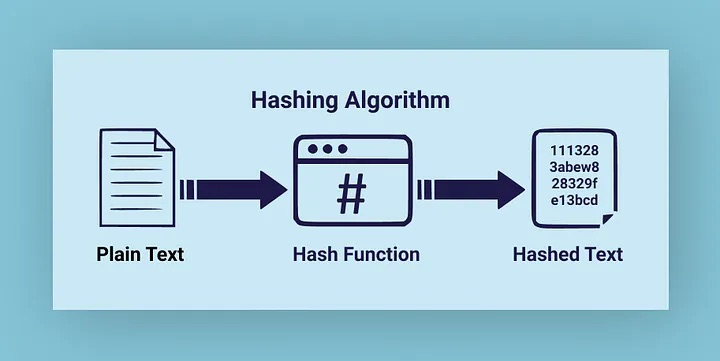
\includegraphics[width=0.5\textwidth]{img/1-img/hash-function.jpeg}
\end{center}
    

\end{frame}


\begin{frame}
\frametitle{Proprietà delle funzioni di hash}

\begin{itemize}
    \item \textbf{Determinismo}: per uno stesso input la funzione restituisce sempre lo stesso output.
    \item \textbf{Velocità}: la funzione deve essere veloce da calcolare.
    \item \textbf{Difficoltà di inversione}: data l'uscita della funzione è computazionalmente difficile trovare l'input.
    \item \textbf{Diffusione}: piccole variazioni nell'input devono produrre grandi variazioni nell'output.
    \item \textbf{Resistenza alle collisioni}: è computazionalmente difficile trovare due input diversi che producano lo stesso output.
\end{itemize}
\end{frame}

\begin{frame}
\frametitle{Preimage resistence}
Prima (debole) resistenza alla preimmagine:
\begin{itemize}
    \item per quasi tutti gli output pre-specificati, è computazionalmente infattibile trovare un qualsiasi input che venga hashato a quell'output.
    Avendo \( y \), è difficile trovare un \( x \) tale che \( h(x) = y \).
\end{itemize}
Seconda (forte) resistenza alla preimmagine:
\begin{itemize}
    \item per un input specificato, è computazionalmente infattibile trovare un altro input che produca lo stesso output.
     Avendo \( x \), è difficile trovare un secondo input \( x' \neq x \) tale che \( h(x) = h(x') \).
\end{itemize}

\end{frame}
